% Correlation
% Correlation matrixes
% Practice
  % Example: QOG dataset
  % Practice session
  % Exercise

\documentclass[t]{beamer}
\usetheme{hkllite}

\title{correlation}
	\author{François Briatte \& Ivaylo Petev}
	\date{Week~\#7}

\begin{document}
	
  \frame[plain]{
		\titlepage\\[7.25em]
		\begin{columns}[T]
			\column{.4\textwidth}
				\tableofcontents[hideallsubsections]
			\column{.5\textwidth}
				\hfill %
				\href{http://replicatedtypo.com/wp-content/uploads/2012/11/ChocolateSerialKillers_WintersRoberts.pdf}%
					{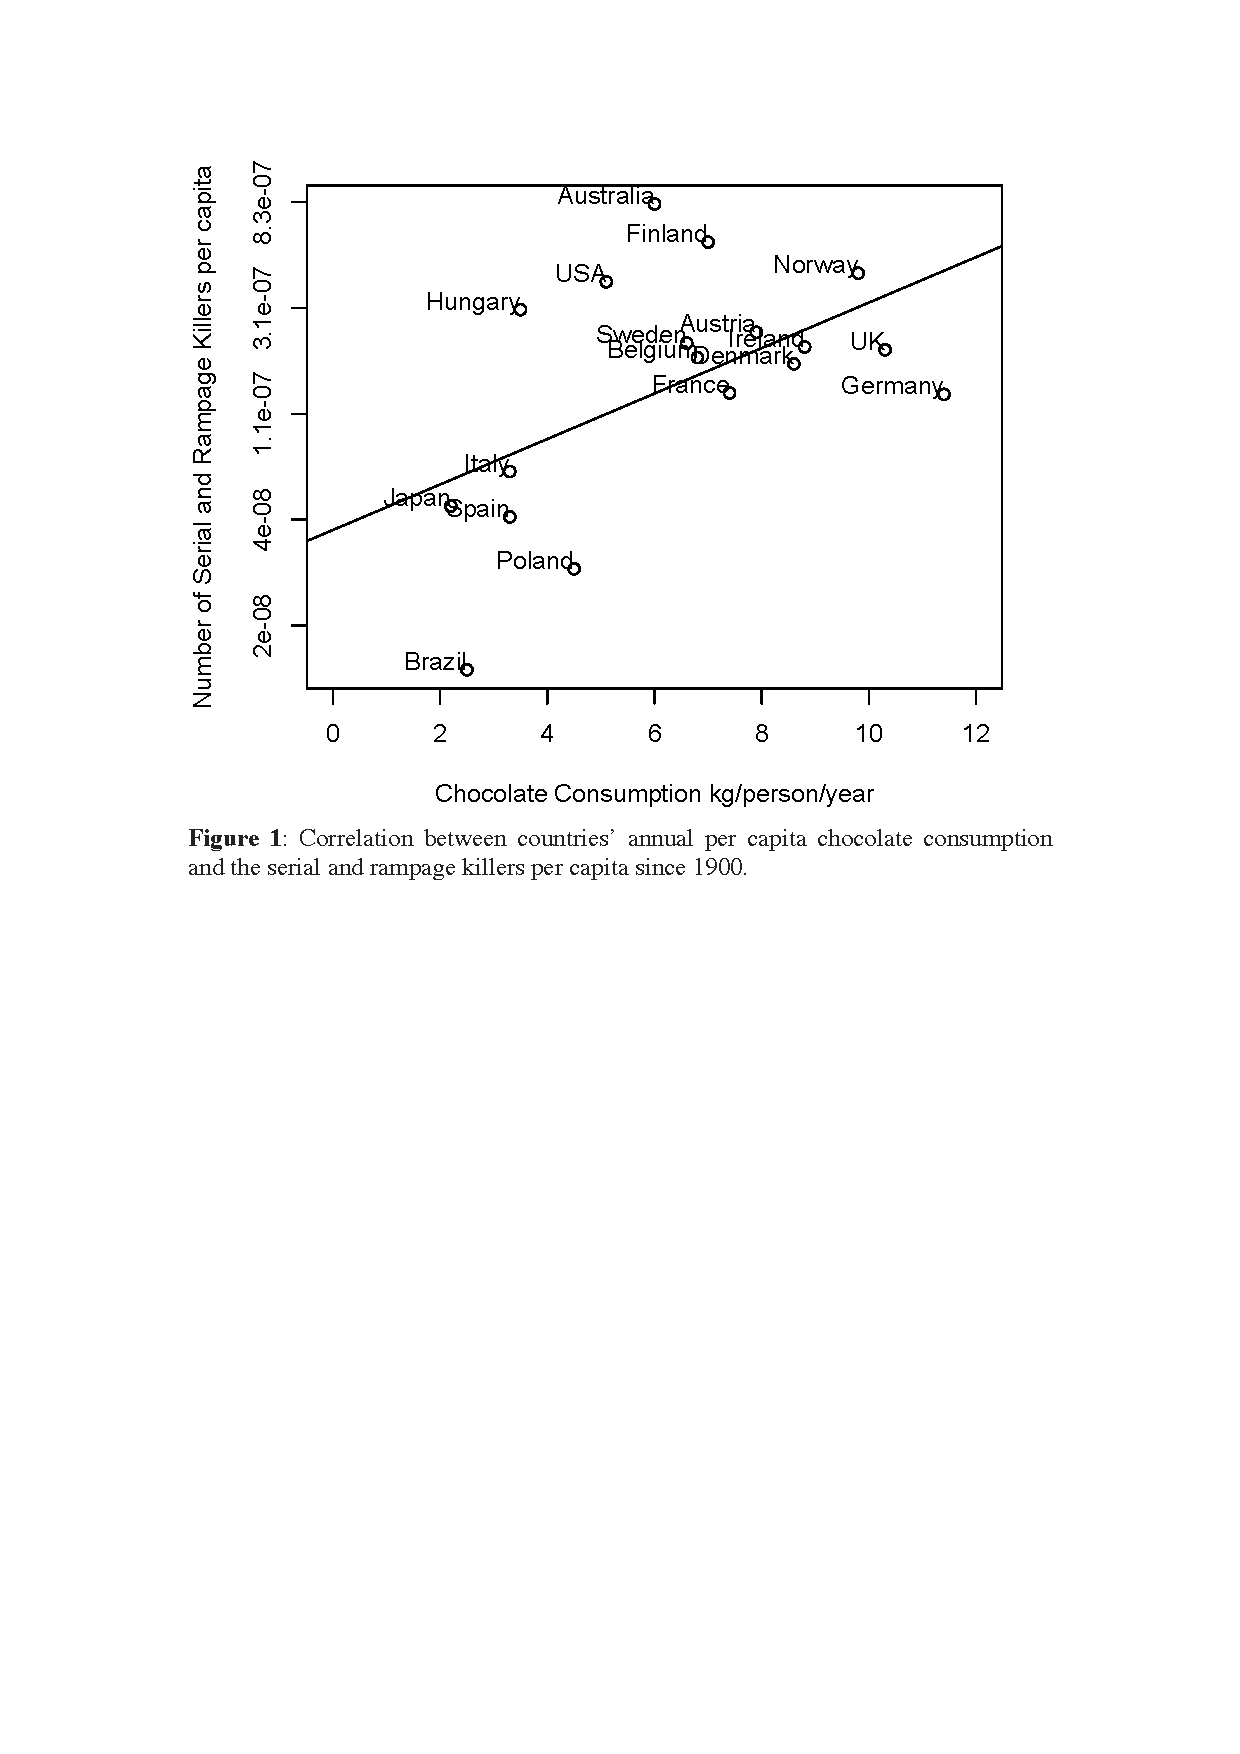
\includegraphics[width=\textwidth]{correlation-chocolate-murders}}		
		\end{columns}
	}
	%
	%
	
	\section{Correlation}
	
    \begin{frame}[c]{\thesection.~Correlation}
	
		\begin{center}
			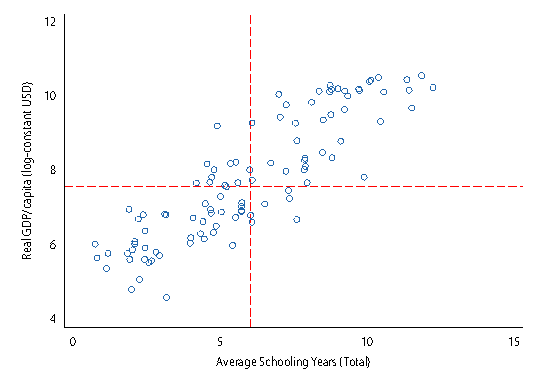
\includegraphics[height=6.5cm]{correlation-scatterplot}
		\end{center}
				
	\end{frame}
	
	\begin{frame}{Pearson correlation coefficient}
	
		\begin{block}{Measuring association as the linear dependence of two variables:}
		
			\begin{align*}
				\text{Population notation} \quad
				\rho &= \frac{\text{Cov}(X,Y)}{\text{Var}_X\text{Var}_Y}, \quad
				-1 \leq \rho \leq 1
				\\
				\text{Sample notation} \quad
				r &= \frac{1}{n-1} \sum ^n _{i=1} (\frac{X_i - \bar{X}}{s_X}) (\frac{Y_i - \bar{Y}}{s_Y})
			\end{align*}

		\end{block}
		
		\begin{alertblock}{Detects linear correlation}

			\begin{itemize}
				\item Uncorrelated $\neq$ unrelated
				\item Correlated $\neq$ unconfounded
			\end{itemize}
						
		\end{alertblock}
					
	\end{frame}

	%
	%

	\begin{frame}[c]{Perfect (positive, negative) correlation}
			
		\begin{center}
			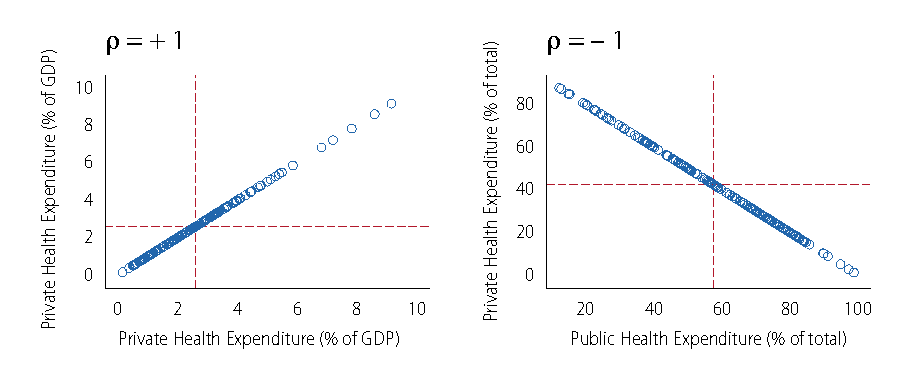
\includegraphics[width=\textwidth]{correlation-perfect}		
		\end{center}

	\end{frame}	

	\begin{frame}[c]{Significant (moderate, strong) correlation}
			
		\begin{center}
			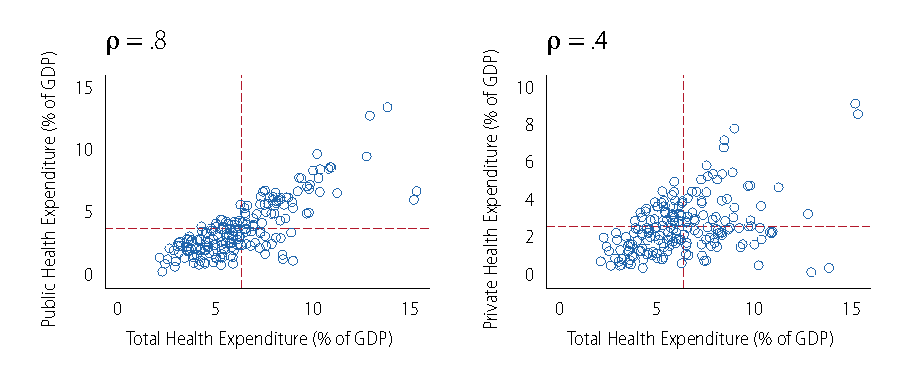
\includegraphics[width=\textwidth]{correlation-significant}		
		\end{center}

	\end{frame}	

	\begin{frame}[c]{Insignificant (weak, non-linear) correlation}
			
		\begin{center}
			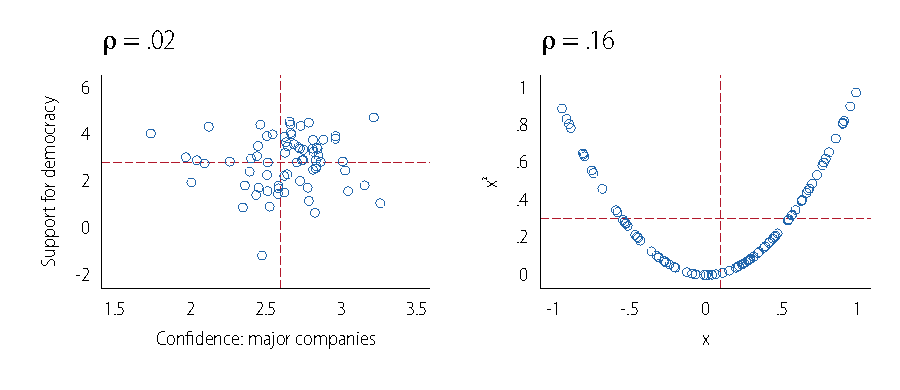
\includegraphics[width=\textwidth]{correlation-insignificant}		
		\end{center}

	\end{frame}
	
	%
	%
	
	\begin{frame}{Pearson correlation coefficient}
	
		\begin{block}{Significance test:}

			\begin{align*}
				\text{Null hypothesis~} H_0 \quad
				r &= 0
				\\
				\text{Test statistic} \quad
				T &= r \sqrt{\frac{n-2}{1-r^2}}
			\end{align*}

		\end{block}
		
		\begin{alertblock}{Sanity check}

			\begin{itemize}
				\item Uncorrelated $\neq$ independent
				\item Correlated $\neq$ causally related
			\end{itemize}
			
		\end{alertblock}
						
	\end{frame}
		
	%
	%
	
    \begin{frame}[c]

		\begin{center}
			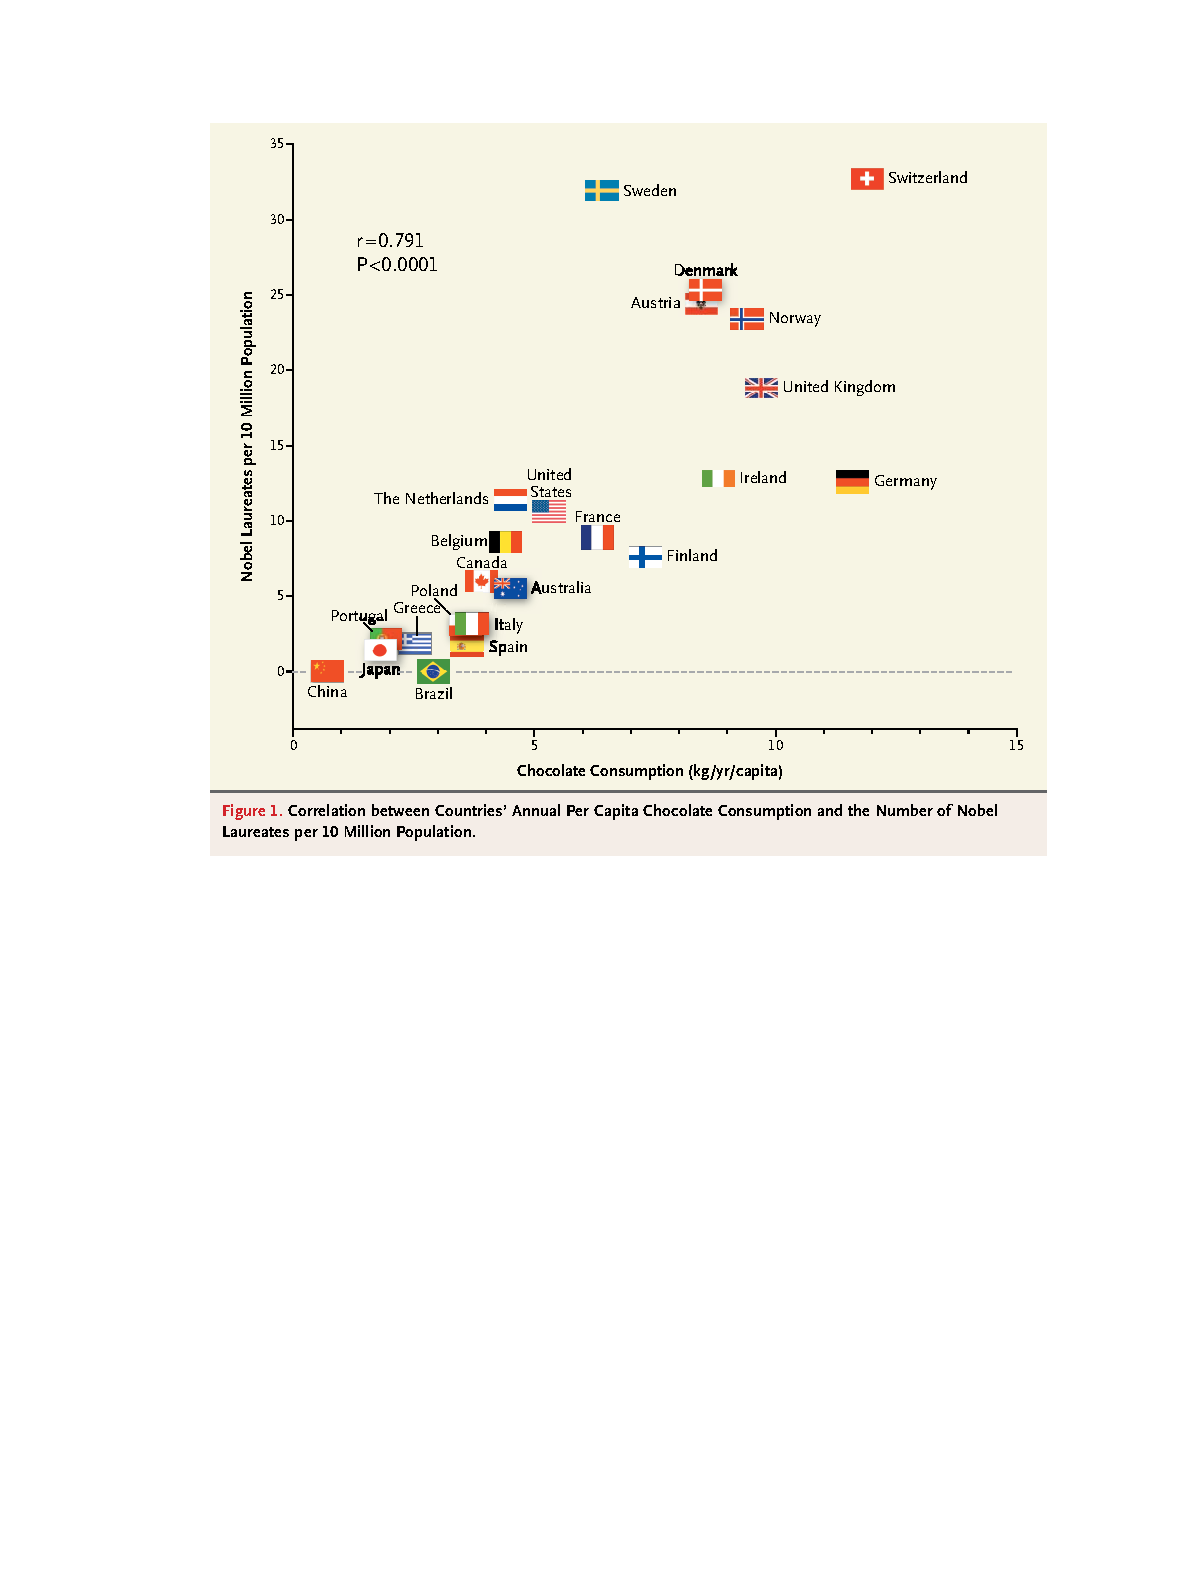
\includegraphics[height=6.5cm]{chocolate-nobel}
		\end{center}
		
		\vfill \par Source: Messerli, ``\href{http://www.nejm.org/doi/pdf/10.1056/NEJMon1211064}{Chocolate Consumption, Cognitive Function, and Nobel Laureates}'', \emph{New England Journal of Medicine}, 2012.
		
	\end{frame}

	%
	%
	
	\begin{frame}[c]

		\begin{center}
			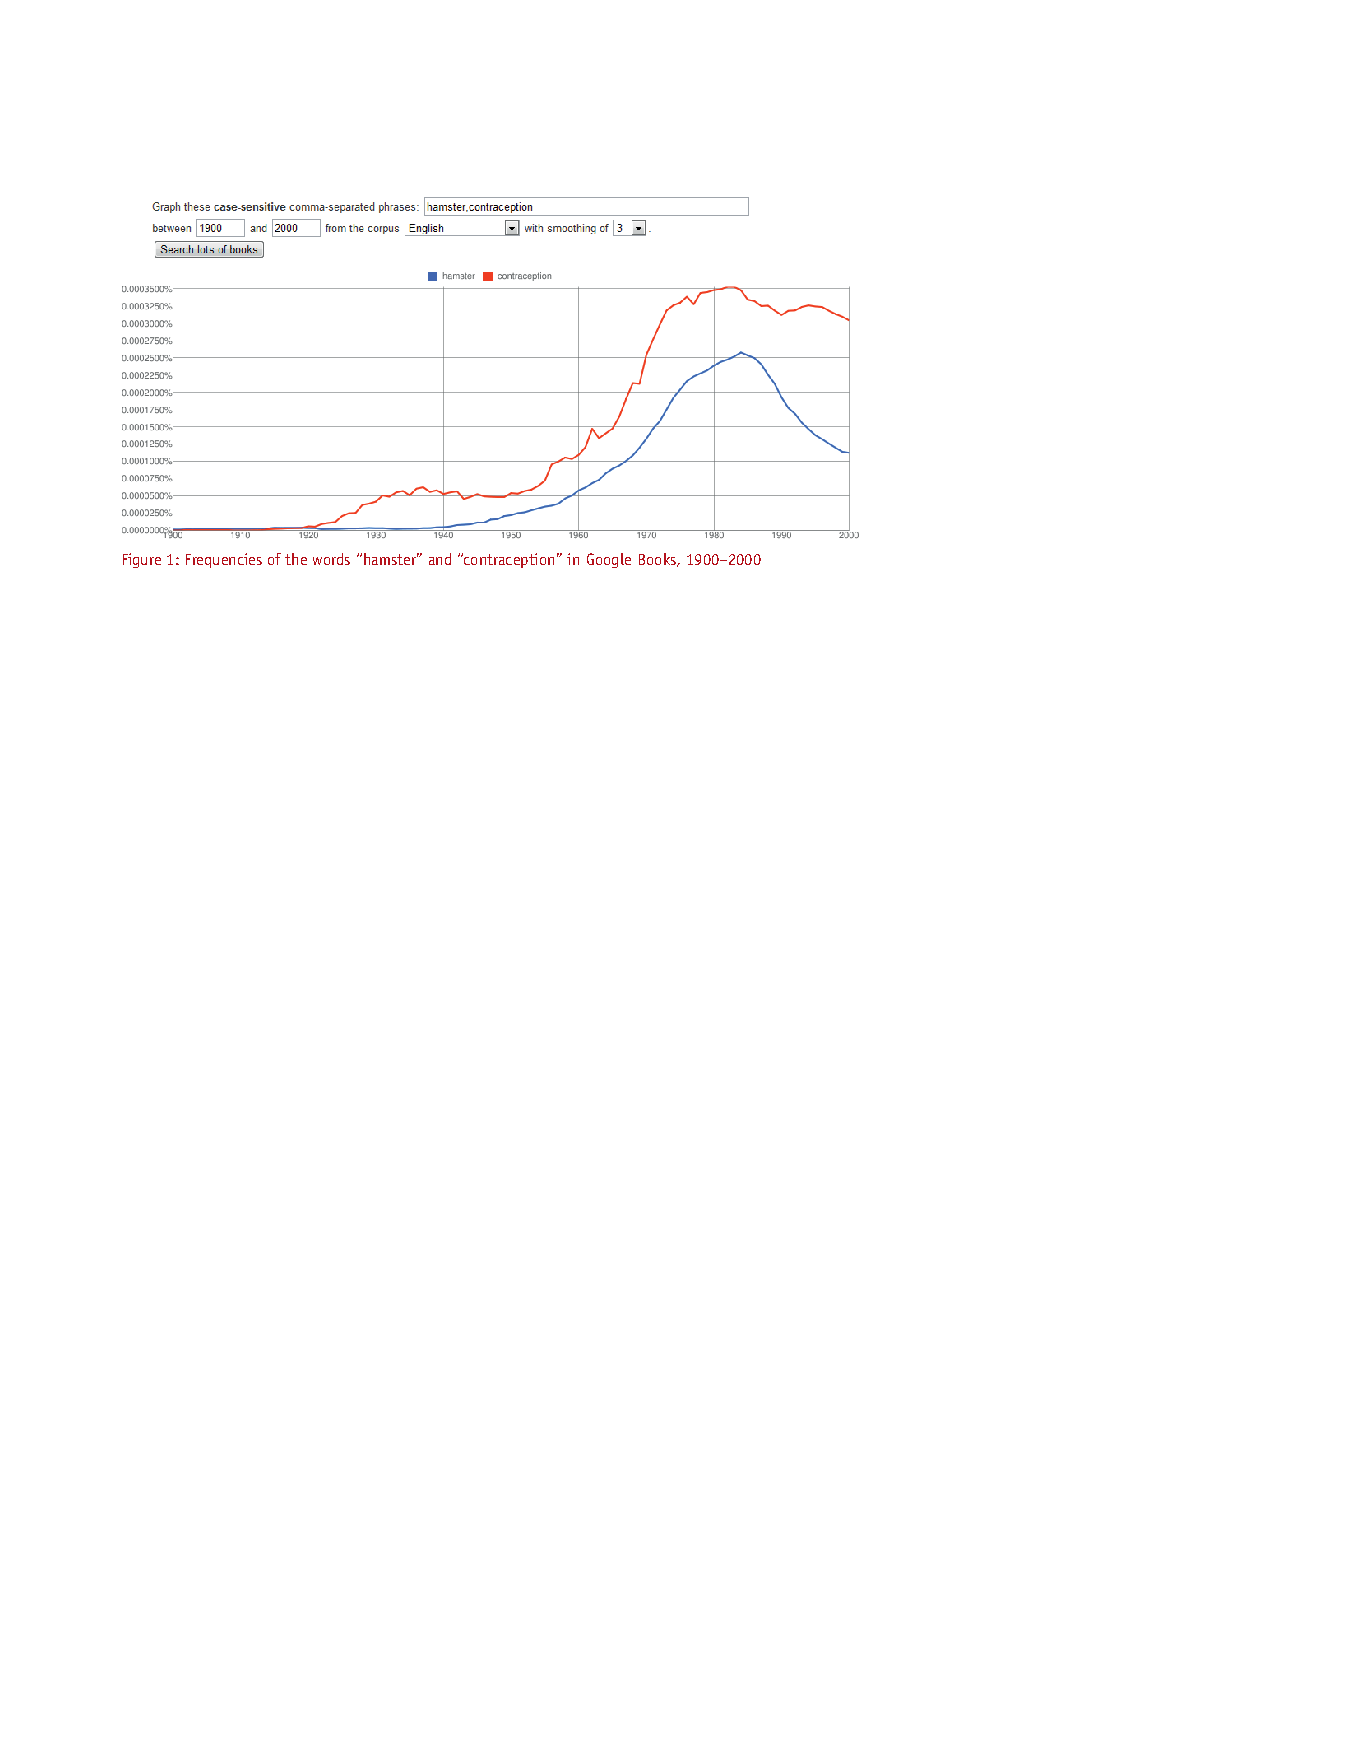
\includegraphics[width=\textwidth]{hamster-contraception}	
		\end{center}
		
		\vfill \par Source: Harkness, ``\href{http://onlinelibrary.wiley.com/doi/10.1111/j.1740-9713.2012.00549.x/abstract}{Seduced by Stats?}'', \emph{Significance}, 2012.
		
	\end{frame}

	%
	%
	
	\section{Correlation matrixes}

  \begin{frame}[c]{\thesection.~Correlation matrixes}
		
		\begin{block}{\texttt{pwcorr [varlist], [obs sig]}}

	        \begin{itemize}
	          \item \texttt{obs} shows the number of observations
			  \item \texttt{sig} shows the coefficient's $p$-value
	        \end{itemize}

		\end{block}

		\begin{block}{\texttt{gr mat [varlist], [half etc.]}}		

	        \begin{itemize}
	          \item \texttt{half} plots only half of all graphs (quicker)
			  		\item accepts scatterplot options (\texttt{jitter}, \texttt{mlab}, etc.)
	        \end{itemize}

		\end{block}
	
	\end{frame}

	%
	%

  \begin{frame}[c]{Correlation matrixes}
	
		\begin{block}{\texttt{mkcorr [varlist], lab num sig log(file.txt) replace}}
			\begin{itemize}
				\item \texttt{ssc install mkcorr} to install
				\item \texttt{help mkcorr} to understand the options
			\end{itemize}
		\end{block}
	
		\begin{alertblock}{Computer skills}
			\begin{itemize}
				\item Import as a table in a spreadsheet editor.
				\item Convert from text to table in a rich text editor.
			\end{itemize}
			  
		\end{alertblock}

	\end{frame}
		
	%
	%

	% \begin{frame}[c]{One variable, many predictors}
	% 
	% 	\begin{center}
	% 		\includegraphics[width=.7\textwidth]{hate-sc1}	
	% 	\end{center}
	% 	
	% 	\par Source: Florida, ``\href{http://www.theatlantic.com/national/archive/2011/05/the-geography-of-hate/238708/}{The Geography of Hate}'', \emph{The Atlantic}, 2011.
	% 	
	% \end{frame}
	% 
	% \begin{frame}[c]{One variable, many predictors}
	% 
	% 	\begin{center}
	% 		\includegraphics[width=.7\textwidth]{hate-sc2}	
	% 	\end{center}
	% 	
	% 	\par Source: Florida, ``\href{http://www.theatlantic.com/national/archive/2011/05/the-geography-of-hate/238708/}{The Geography of Hate}'', \emph{The Atlantic}, 2011.
	% 	
	% \end{frame}
	% 
	% \begin{frame}[c]{One variable, many predictors}
	% 
	% 	\begin{center}
	% 		\includegraphics[width=.7\textwidth]{hate-sc3}	
	% 	\end{center}
	% 	
	% 	\par Source: Florida, ``\href{http://www.theatlantic.com/national/archive/2011/05/the-geography-of-hate/238708/}{The Geography of Hate}'', \emph{The Atlantic}, 2011.
	% 	
	% \end{frame}
	% 
	% \begin{frame}[c]{One variable, many predictors}
	% 
	% 	\begin{center}
	% 		\includegraphics[width=.7\textwidth]{hate-sc4}	
	% 	\end{center}
	% 	
	% 	\par Source: Florida, ``\href{http://www.theatlantic.com/national/archive/2011/05/the-geography-of-hate/238708/}{The Geography of Hate}'', \emph{The Atlantic}, 2011.
	% 	
	% \end{frame}
	% 
	% \begin{frame}[c]{One variable, many predictors}
	% 
	% 	\begin{center}
	% 		\includegraphics[width=.7\textwidth]{hate-sc5}	
	% 	\end{center}
	% 	
	% 	\par Source: Florida, ``\href{http://www.theatlantic.com/national/archive/2011/05/the-geography-of-hate/238708/}{The Geography of Hate}'', \emph{The Atlantic}, 2011.
	% 	
	% \end{frame}

	%
	%

	\begin{frame}[c]{\texttt{gr mat}}

		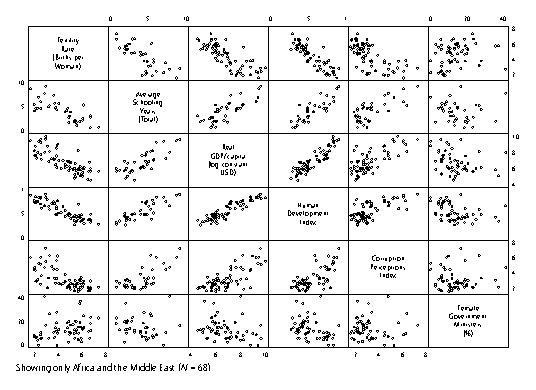
\includegraphics[width=\textwidth]{correlation-matrix}
				
	\end{frame}
	
	\begin{frame}[t]{From Stata output...}

		\begin{tikzpicture}
			\node[anchor=south west,inner sep=0] (image) at (0,0) {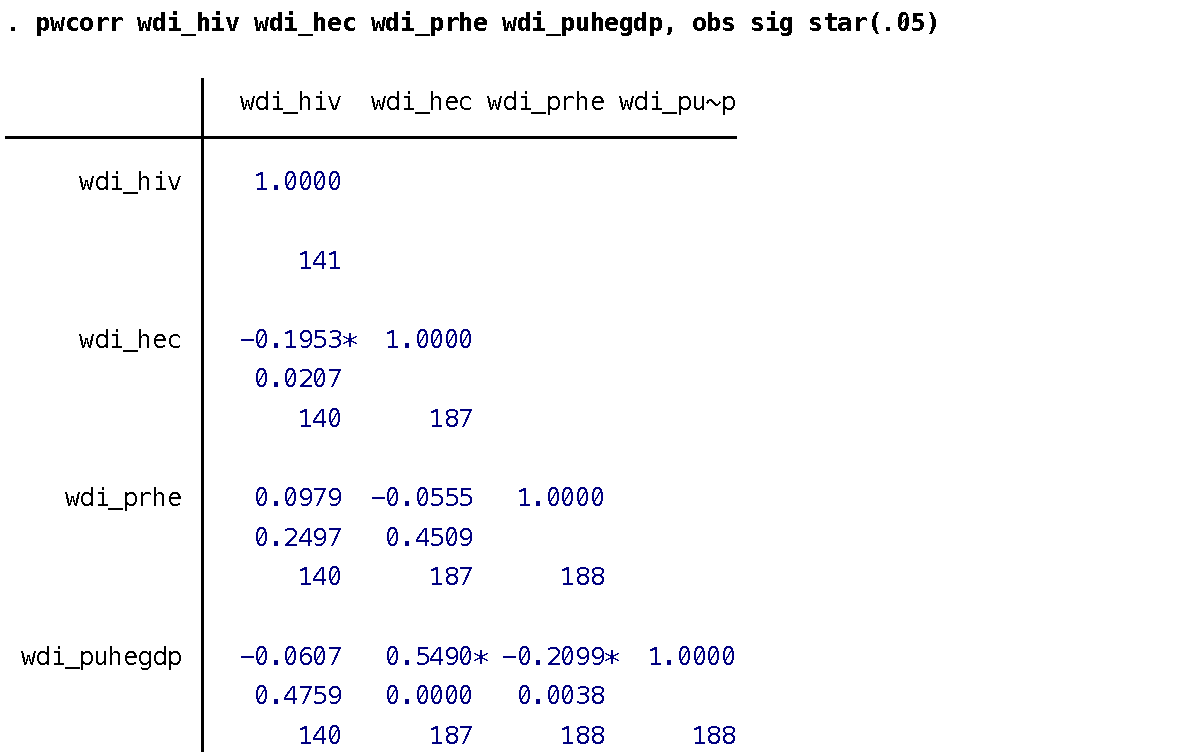
\includegraphics[width=.8\textwidth]{pwcorr}};
			
		    \begin{scope}[x={(image.south east)},y={(image.north west)}]
				\draw[fill=blue, opacity=0.25] (.32, .11) rectangle (.42, .17);
				\draw[fill=red, opacity=0.25] (.43, .05) rectangle (.53, .11);
				\draw[fill=green, opacity=0.25] (.54, -.01) rectangle (.64, .05);
		    		\node[anchor=west, fill=blue, text opacity=1, opacity=0.25] at (.8, .22) { coefficient };
		    		\node[anchor=west, fill=red, text opacity=1, opacity=0.25] at (.8, .10) { $p$-value };
		    		\node[anchor=west, fill=green, text opacity=1, opacity=0.25] at (.8, -.02) { observations };
%				\draw[help lines,xstep=.1,ystep=.1] (0,0) grid (1,1);
%				\foreach \x in {0,1,...,9} { \node [anchor=north] at (\x/10,0) {0.\x}; }
%				\foreach \y in {0,1,...,9} { \node [anchor=east] at (0,\y/10) {0.\y}; }
				\draw[fill=yellow, opacity=0.25] (.19, .42) rectangle (.31, .58);
		    		\node[anchor=west, fill=yellow, text opacity=1, align=left, opacity=0.25] at (.8, .58) { $r = -.2$ \\ $p < .02$ \\ $N = 140$ };
		    \end{scope}
		\end{tikzpicture}
			
	\end{frame}

	\begin{frame}[t]{... to publishing standard}

		\begin{center}
			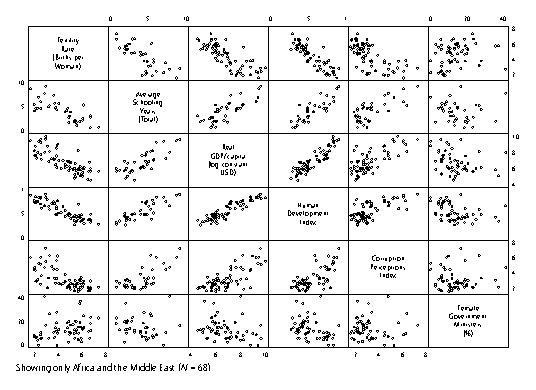
\includegraphics[width=\textwidth]{correlation-matrix}	
		\end{center}
		
		\vfill \par Source: Adhikari \emph{et al.}, ``Public Policy, Political Connections, and Effective Tax Rates: Longitudinal Evidence from Malaysia'', \emph{Journal of Accounting and Public Policy}, 2006.
		
	\end{frame}
	%
	%

	%
	%
	\section{Practice}
	%	
	%

	%
	%
	\subsection{Example: QOG dataset}
	%
	%
	
	\begin{frame}[t]{Practice: \red{QOG dataset}}

		\begin{columns}[c]
			\column{.55\textwidth}

	    Data:\\[.5em]

			\begin{itemize}
				\item Quality of Government (QOG)
				\item Sample: countries, c.~2002
			\end{itemize}
		
			\vspace{.75em}
		
	    Variables:\\[.5em]
		
			\begin{itemize}
				\item Fertility rate
				\item Education years
				\item Corruption Perceptions Index
				\item Human Development Index
				\item Female ministers
			\end{itemize}
	
			\column{.35\textwidth}

			
\includegraphics[width=\textwidth]{logo-qog}

		\end{columns}
	
	\end{frame}
	%
	%
	
	%
	%
	\subsection{Practice session}
  %
  %
  
	\begin{frame}[t]{Practice session}

    \begin{block}{Class}
      \comm{Get the do-file for this week.}\\
      \code{srqm\_get week7.do}\\
      
			\comm{Open to read and replicate.}\\
			\code{doedit code/week7}\\    
    \end{block}

    \begin{alertblock}{Coursework}
      \begin{itemize}
	      \item Finish the do-file and read all comments at home.
	      \item Correct your do-file and add significance tests.
	      \item Correct your paper and substantiate its hypotheses.
      \end{itemize}
    \end{alertblock}
    		
	\end{frame}
  %
  %
		
\end{document}
